\documentclass[11pt,a4paper]{article}
\usepackage{fontspec}
\setmainfont{texgyretermes}[Extension=.otf,UprightFont=*-regular,BoldFont=*-bold,ItalicFont=*-italic,BoldItalicFont=*-bolditalic]
\setsansfont{texgyreheros}[Extension=.otf,UprightFont=*-regular,BoldFont=*-bold,ItalicFont=*-italic,BoldItalicFont=*-bolditalic]
\setmonofont{lmmono10}[Extension=.otf,UprightFont=*-regular]
\usepackage[a4paper,margin=2.2cm]{geometry}
\usepackage{graphicx,booktabs,tabularx,array,amsmath,amssymb,float,enumitem,xcolor}
\usepackage[font=small,labelfont=bf]{caption}
\usepackage{tikz}
\usetikzlibrary{positioning,arrows.meta,shapes.geometric,fit,backgrounds}
\usepackage[most]{tcolorbox}
\usepackage[colorlinks=true,linkcolor=teal!60!black,urlcolor=teal!60!black]{hyperref}
\usepackage{titlesec}

\definecolor{mk}{HTML}{4C72B0}
\definecolor{pa}{HTML}{DD8452}
\definecolor{pe}{HTML}{55A868}
\definecolor{acc}{HTML}{2A9D8F}
\titleformat{\section}{\Large\sffamily\bfseries\color{teal!50!black}}{\thesection}{0.6em}{}
\titleformat{\subsection}{\large\sffamily\bfseries}{\thesubsection}{0.5em}{}
\setlist{itemsep=2pt,topsep=3pt}
\renewcommand{\arraystretch}{1.2}

\newtcolorbox{ghichu}[1][Điểm cần nhớ]{colback=acc!6,colframe=acc!70!black,fonttitle=\sffamily\bfseries,title=#1,
  boxrule=0.6pt,arc=2pt,left=6pt,right=6pt,top=4pt,bottom=4pt}

\captionsetup{justification=raggedright,singlelinecheck=false}
\graphicspath{{figs/}}
\renewcommand{\figurename}{Hình}
\renewcommand{\tablename}{Bảng}
\setcounter{topnumber}{3}\setcounter{totalnumber}{4}\renewcommand{\topfraction}{0.9}\renewcommand{\textfraction}{0.1}\renewcommand{\floatpagefraction}{0.75}

\begin{document}

\begin{center}
{\sffamily\bfseries\LARGE UPAR Challenge 2027 \textendash{} Track 1\\[3pt]
\Large Pedestrian Attribute Recognition}\\[8pt]
{\large Báo cáo tình hình: bài toán, dữ liệu, cách chấm điểm và vấn đề cần giải quyết}\\[6pt]
{\small Cập nhật ngày 28/09/2026 \quad Tài khoản Codabench \texttt{tannguyenbmt47}}
\end{center}

\begin{ghichu}[Tóm tắt]
\begin{itemize}[leftmargin=1.2em]
\item Cho một ảnh crop của một người đi bộ, mô hình phải trả về 40 xác suất cho 40 thuộc tính nhị phân như tuổi, giới tính, độ dài tóc, màu và kiểu quần áo, phụ kiện.
\item Mô hình được huấn luyện trên ba bộ dữ liệu công khai (Market1501, PA100k, PETA) nhưng được chấm trên một bộ test ẩn đến từ domain chưa từng thấy. Đây là bài toán tổng quát hoá qua domain.
\item Bài nộp là code. Server của ban tổ chức chạy \texttt{run.py} trong container không có mạng, giới hạn 1 giờ, và không trả log cho người tham gia.
\item Mô hình hiện tại (DINOv3 ViT-B/16) đạt Challenge\_Avg 0.885 trên val cùng domain nhưng chỉ 0.777 trên test. Khoảng chênh 0.108 là thước đo trực tiếp của vấn đề domain shift.
\item Trên leaderboard ngày 28/09/2026, bài nộp xếp thứ 2 với 0.7774, kém vị trí đầu (0.7779) 0.0005 điểm.
\end{itemize}
\end{ghichu}

\section{Bối cảnh cuộc thi}

UPAR Challenge là cuộc thi đi kèm workshop Real-World Surveillance (RWS) tại WACV. Kỳ 2027 là lần tổ chức thứ ba, sau hai kỳ 2023 và 2024. Kỳ 2025 và 2026 của workshop tổ chức challenge khác về ảnh nhiệt. Track 1 là nhận dạng thuộc tính người đi bộ (Pedestrian Attribute Recognition, PAR). Track 2 là truy vấn người theo thuộc tính, dùng chung bộ 40 thuộc tính.

\begin{table}[H]
\centering\small
\begin{tabularx}{\linewidth}{@{}lX@{}}
\toprule
Hạng mục & Nội dung \\
\midrule
Hạn nộp bài & 21/10/2026 AoE. Hạn nộp paper là 23/10, hạn nộp code để kiểm chứng là 30/10 \\
Lượt nộp & 3 lượt mỗi ngày, tổng cộng 50 lượt. Leaderboard hiển thị bài nộp mới nhất, không phải bài tốt nhất \\
Môi trường chạy & Docker \texttt{pytorch/pytorch:2.4.1-cuda12.1-cudnn9-runtime}, Python 3.11, không có mạng, giới hạn 3600 giây. Phần cứng không được công bố \\
Dữ liệu được dùng & Chỉ dữ liệu ban tổ chức cung cấp. Được dùng model pretrain chung như ImageNet, DINOv3, CLIP. Cấm dữ liệu PAR bên ngoài \\
Ảnh test & Cấm dùng dưới mọi hình thức, gồm huấn luyện, pseudo-label, gán nhãn tay và chọn siêu tham số \\
Điều kiện thắng & Vượt baseline của ban tổ chức và nộp code, trọng số, fact sheet để kiểm chứng \\
\bottomrule
\end{tabularx}
\caption{Các quy định chính của Track 1, tổng hợp từ trang Codabench của cuộc thi.}
\end{table}

\section{Bài toán: input và output}

\subsection{Luồng chấm bài}

Người tham gia không nộp file kết quả. Họ nộp một file zip chứa \texttt{run.py}, trọng số và mọi thư viện cần thiết. Hình~\ref{fig:pipeline} mô tả luồng xử lý trên server.

\begin{figure}[!htb]
\centering
\begin{tikzpicture}[
  node distance=5mm and 6mm,
  box/.style={draw, rounded corners=2pt, align=center, font=\small\sffamily, minimum height=13mm, text width=26mm, fill=#1},
  box/.default=white, >={Stealth[length=2.2mm]}]
\node[box=gray!10] (data) {Ảnh test ẩn\\\footnotesize domain chưa thấy\\\footnotesize images.csv, task.json};
\node[box=gray!10, right=of data] (ing) {Ingestion\\\footnotesize gọi \texttt{load\_model()}\\\footnotesize và \texttt{predict\_batch()}};
\node[box=acc!15, right=of ing] (run) {\texttt{run.py} của đội\\\footnotesize ảnh $\rightarrow$ model\\\footnotesize $\rightarrow$ 40 xác suất};
\node[box=gray!10, right=of run] (thr) {Ngưỡng cố định\\\footnotesize $p > 0.5 \Rightarrow 1$\\\footnotesize ngược lại 0};
\node[box=gray!10, below=9mm of thr] (score) {Scoring\\\footnotesize mA, Instance-F1\\\footnotesize theo từng dataset};
\node[box=orange!15, left=of score] (lb) {Leaderboard\\\footnotesize Challenge\_Avg};
\draw[->] (data) -- (ing); \draw[->] (ing) -- (run); \draw[->] (run) -- (thr); \draw[->] (thr) -- (score); \draw[->] (score) -- (lb);
\begin{scope}[on background layer]
\node[draw=red!60, dashed, rounded corners, fit=(ing)(run), inner sep=5pt, label={[font=\footnotesize\sffamily,red!70!black]above:container Docker, không mạng, tối đa 3600 giây, log bị ẩn}] {};
\end{scope}
\end{tikzpicture}
\caption{Luồng chấm bài của Track 1. Phần duy nhất đội thi kiểm soát là \texttt{run.py} và các file đi kèm. Ngưỡng 0.5 do ban tổ chức cố định nên mọi hiệu chỉnh ngưỡng phải thực hiện bên trong \texttt{run.py}.}
\label{fig:pipeline}
\end{figure}

\subsection{Input}

Với mỗi ảnh test, ingestion program truyền cho \texttt{run.py} một dict gồm chỉ số ảnh, đường dẫn tương đối, đường dẫn tuyệt đối và danh sách 40 tên thuộc tính. Ảnh là crop RGB chứa một người, đã được cắt sẵn từ camera giám sát. Đội thi không phải phát hiện người. Kích thước ảnh không cố định. Trong dữ liệu train, ảnh Market1501 luôn là 64×128 pixel, ảnh PA100k có trung vị 74×202 pixel và ảnh PETA có trung vị 73×160 pixel. Có 244 ảnh cao dưới 60 pixel.

\subsection{Output}

Với mỗi ảnh, \texttt{run.py} trả về một vector 40 số thực trong khoảng $[0,1]$, theo đúng thứ tự tên thuộc tính. Giá trị lớn hơn 0.5 được coi là thuộc tính có mặt. Một giá trị NaN, một giá trị ngoài $[0,1]$ hoặc một vector sai độ dài làm toàn bộ bài nộp thất bại. Đây là bài toán phân loại đa nhãn. Một ảnh có trung bình khoảng 7 nhãn dương.

\begin{table}[H]
\centering\small
\begin{tabularx}{\linewidth}{@{}l c X l@{}}
\toprule
Nhóm & Chỉ số & Thuộc tính & Quan hệ trong nhóm \\
\midrule
Tuổi & 0--2 & Young, Adult, Old & gần như chọn 1 trong 3 \\
Giới tính & 3 & Female & nhị phân \\
Tóc & 4--6 & Short, Long, Bald & gần như chọn 1 trong 3 \\
Áo & 7 & UpperBody-Length-Short (cộc tay) & nhị phân \\
 & 8--19 & 12 màu: Black, Blue, Brown, Green, Grey, Orange, Pink, Purple, Red, White, Yellow, Other & thường 1 màu \\
Quần & 20 & LowerBody-Length-Short (quần hoặc váy ngắn) & nhị phân \\
 & 21--32 & 12 màu, cùng danh sách với áo & thường 1 màu \\
 & 33--34 & Trousers\&Shorts, Skirt\&Dress & chọn 1 trong 2 \\
Phụ kiện & 35--39 & Backpack, Bag, Glasses-Normal, Glasses-Sun, Hat & độc lập \\
\bottomrule
\end{tabularx}
\caption{40 thuộc tính của Track 1 theo thứ tự output. Nhiều nhóm gần như loại trừ nhau nhưng vẫn được chấm như 40 nhãn độc lập.}
\end{table}

Hình~\ref{fig:io} minh hoạ output thật của mô hình hiện tại trên ba ảnh, mỗi ảnh lấy từ một dataset. Cột xanh là các thuộc tính có nhãn đúng bằng 1. Mô hình dự đoán đúng phần lớn thuộc tính. Ở ảnh PA100k, thuộc tính Accessory-Bag có xác suất 0.59 dù nhãn là 0, nên bị tính là một lỗi dương tính giả.

\begin{figure}[!htb]
\centering
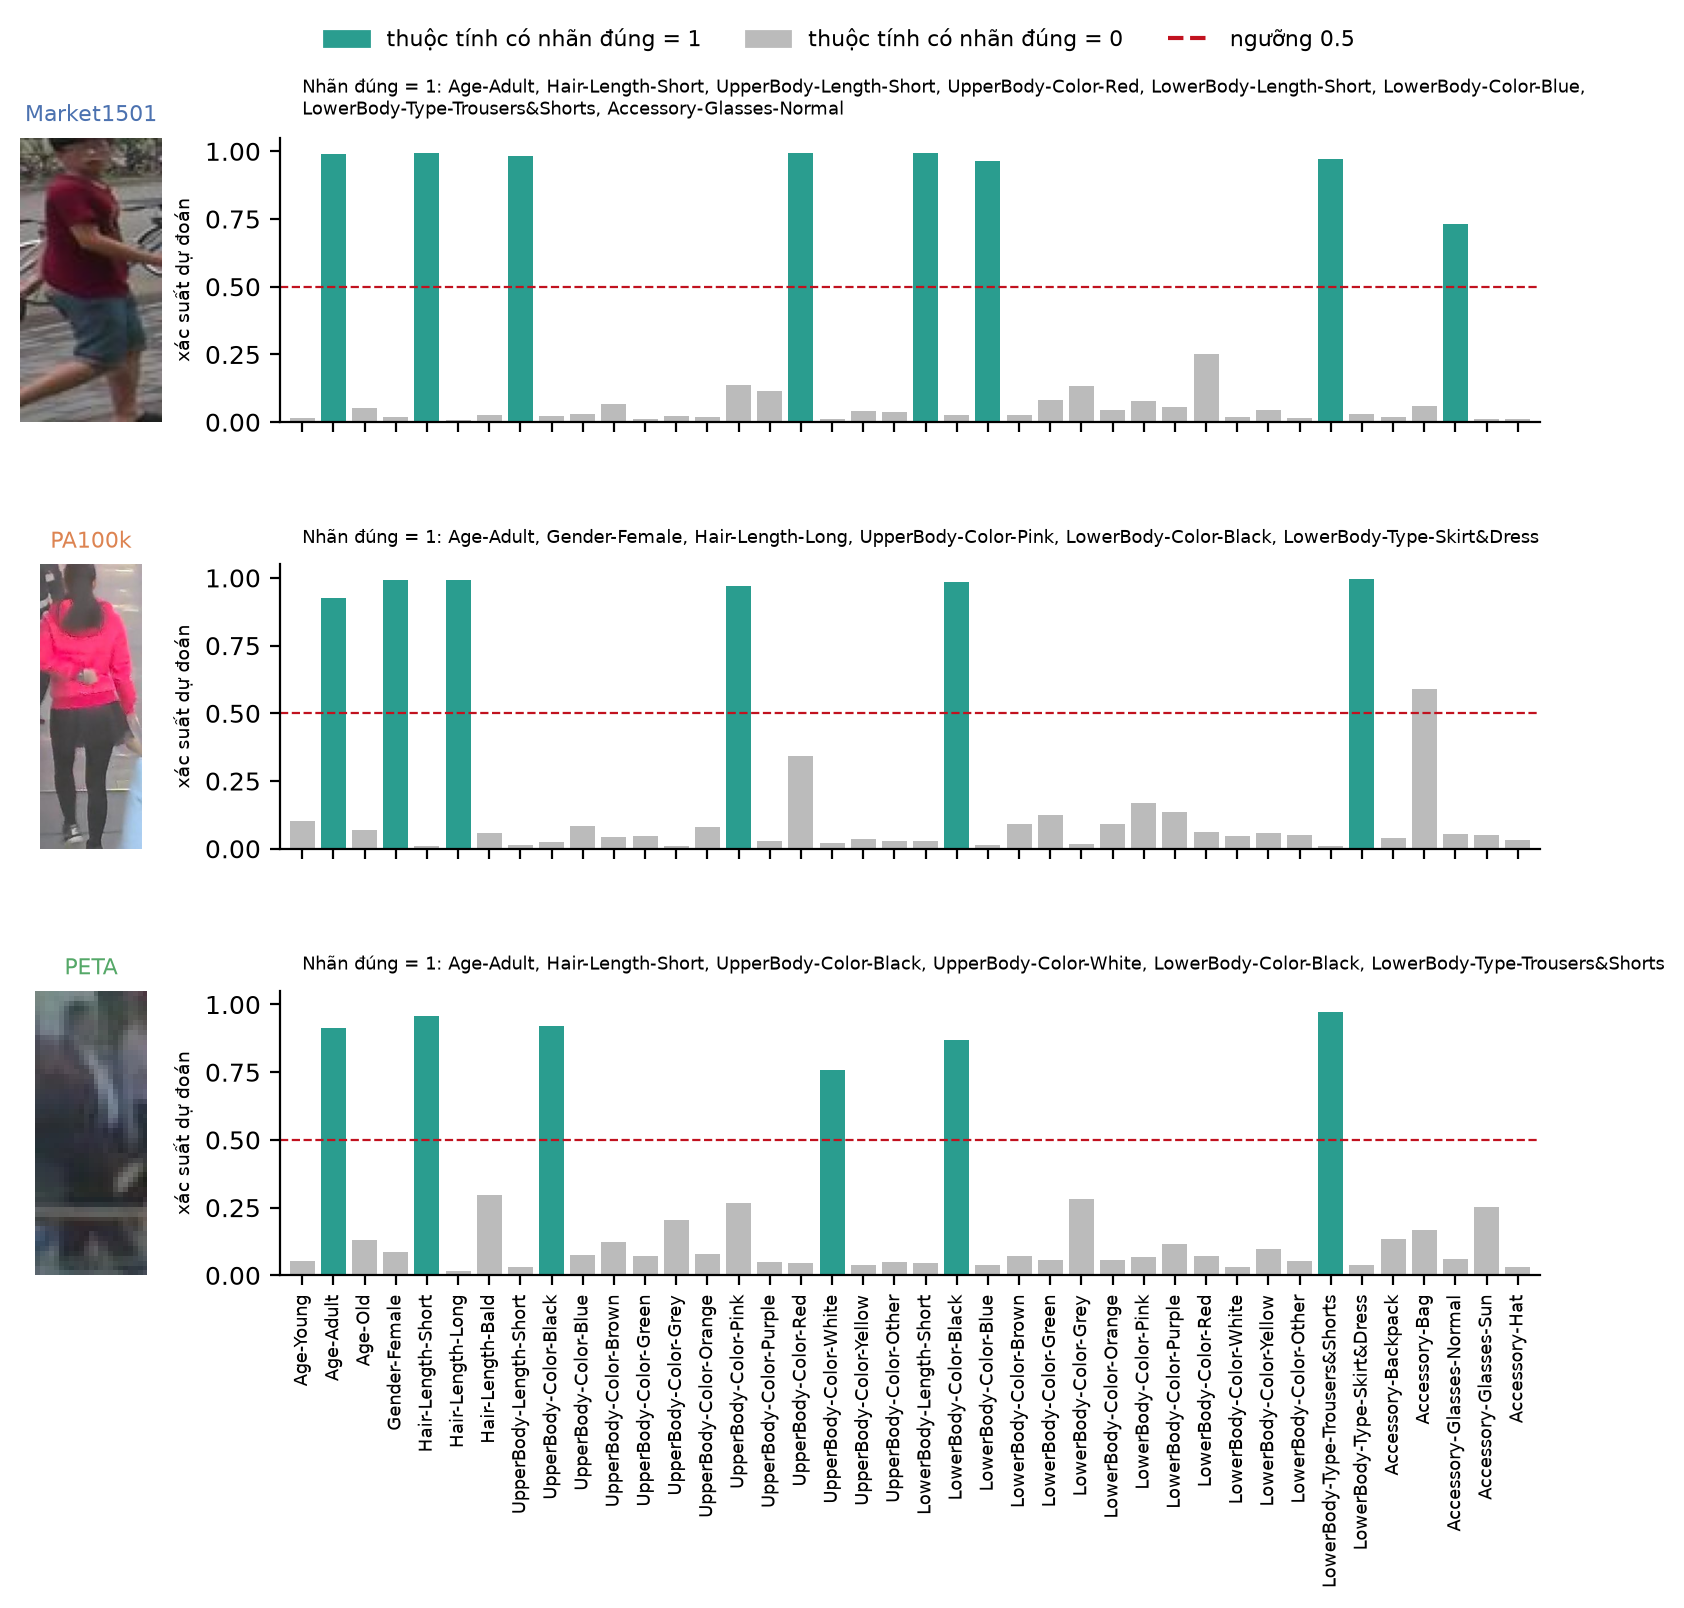
\includegraphics[width=\linewidth]{io_example.png}
\caption{Input và output của bài toán trên ba ảnh thật. Mỗi ảnh cho ra 40 xác suất. Đường đỏ là ngưỡng 0.5 cố định mà hệ thống chấm dùng để chuyển xác suất thành nhãn 0 hoặc 1.}
\label{fig:io}
\end{figure}

\section{Cách chấm điểm}

Hệ thống chấm dùng lại script của kỳ 2024 và tính hai nhóm chỉ số. Gọi $N$ là số ảnh, $A$ là số thuộc tính, $y_{ia}$ là nhãn đúng và $\hat y_{ia}$ là nhãn dự đoán sau ngưỡng 0.5.

\paragraph{Chỉ số theo thuộc tính.} mA tính balanced accuracy riêng cho từng thuộc tính rồi lấy trung bình. Vì mỗi thuộc tính có trọng số như nhau, thuộc tính hiếm như LowerBody-Color-Purple (0.2\% ảnh) nặng ngang thuộc tính phổ biến như Age-Adult (93.5\% ảnh).
\[
\mathrm{mA} = \frac{1}{A}\sum_{a=1}^{A}\frac{1}{2}\left(\frac{TP_a}{TP_a+FN_a}+\frac{TN_a}{TN_a+FP_a}\right)
\]
Số hạng đầu là tỉ lệ bắt được mẫu dương, số hạng sau là tỉ lệ bắt được mẫu âm. Một mô hình không bao giờ dự đoán thuộc tính hiếm sẽ có số hạng đầu bằng 0 và chỉ được 0.5 cho thuộc tính đó.

\paragraph{Chỉ số theo ảnh.} Instance-F1 so sánh tập thuộc tính dự đoán $P_i$ với tập thuộc tính đúng $G_i$ trên từng ảnh, rồi lấy trung bình trên các ảnh.
\[
\mathrm{Prec}_i=\frac{|P_i\cap G_i|}{|P_i|},\quad \mathrm{Rec}_i=\frac{|P_i\cap G_i|}{|G_i|},\quad
\mathrm{F1}_i=\frac{2\,\mathrm{Prec}_i\,\mathrm{Rec}_i}{\mathrm{Prec}_i+\mathrm{Rec}_i}
\]
Chỉ số này phạt mỗi thuộc tính dự đoán thừa. Nó ngược chiều với mA, vì hạ ngưỡng cho thuộc tính hiếm làm mA tăng nhưng sinh thêm dự đoán thừa.

\paragraph{Điểm xếp hạng.} Challenge\_Avg là trung bình điều hoà của mA và Instance-F1. Nếu test gồm nhiều dataset, mỗi dataset được chấm riêng rồi lấy trung bình, nên dataset nhỏ nặng ngang dataset lớn. Thuộc tính không được gán nhãn trong một dataset bị loại khỏi phần chấm của dataset đó.
\[
\mathrm{Challenge\_Avg}=\frac{2\cdot\mathrm{mA}\cdot\mathrm{F1}}{\mathrm{mA}+\mathrm{F1}}
\]

\begin{ghichu}
Ngưỡng 0.5 bị cố định nhưng xác suất do đội thi tự sinh ra. Mọi đánh đổi giữa mA và Instance-F1 được điều khiển bằng cách dịch logit của từng thuộc tính trước khi trả về. Kỳ 2024, một đội dò ngưỡng để tối đa mA và đạt mA cao nhất bảng (72.2) nhưng F1 tụt còn 68.9 và xếp thứ 7.
\end{ghichu}

\section{Dữ liệu}

\subsection{Thành phần và nguồn gốc}

Ban tổ chức cung cấp 97,669 ảnh train và 33,407 ảnh val, cùng định dạng \texttt{gt.csv} gồm đường dẫn ảnh và 40 cột nhãn 0/1. Cả hai tập đến từ ba dataset công khai được chuẩn hoá về chung bộ 40 thuộc tính (Hình~\ref{fig:comp}). Tập train lệch mạnh về PA100k (81\%), còn tập val lệch về Market1501 (49\%). Không có ảnh nào và không có ID người Market nào xuất hiện ở cả hai tập.

\begin{figure}[!htb]
\centering
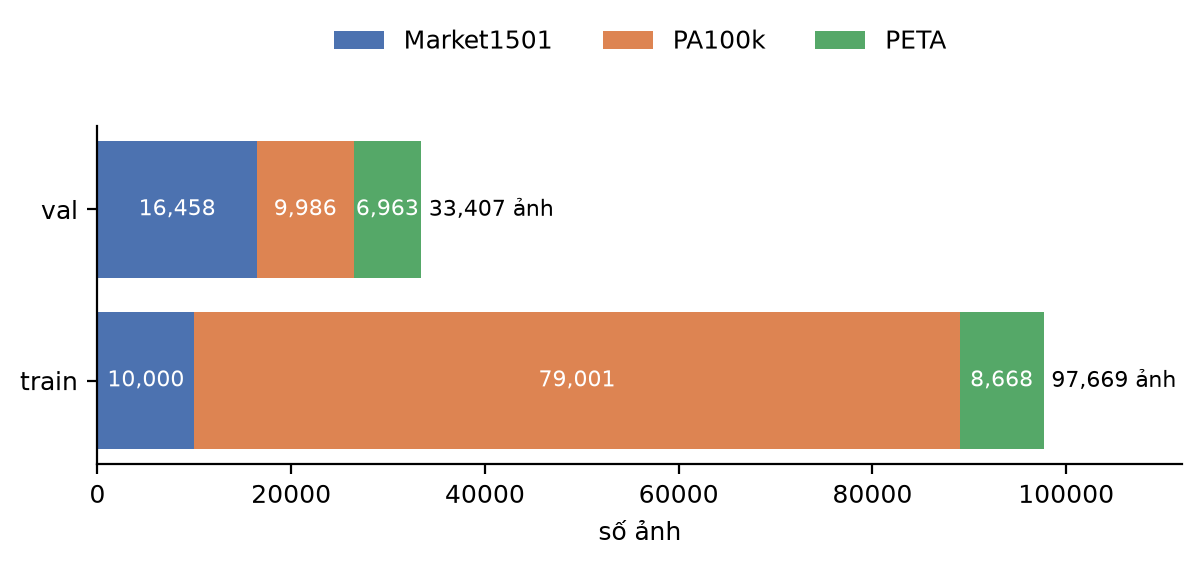
\includegraphics[width=0.8\linewidth]{composition.png}
\caption{Số ảnh của từng dataset trong train và val. PA100k chiếm 81\% tập train nên nếu lấy mẫu đều theo ảnh, mô hình sẽ học chủ yếu đặc thù camera của PA100k.}
\label{fig:comp}
\end{figure}

Market1501 có 1,501 người, mỗi người trung bình 17.6 ảnh. Phần lớn nhãn Market được gán theo người nên mọi ảnh của cùng một người có nhãn giống nhau. Riêng kính và tóc được gán theo từng ảnh vì phụ thuộc góc nhìn. PETA gồm 10 bộ dữ liệu con từ 10 hệ camera khác nhau (TownCentre, CUHK, VIPeR, GRID, CAVIAR4REID, 3DPeS, MIT, PRID, SARC3D, i-LID), nên bản thân PETA đã rất đa dạng về domain.

\subsection{Hình dáng ảnh}

\begin{figure}[!htb]
\centering
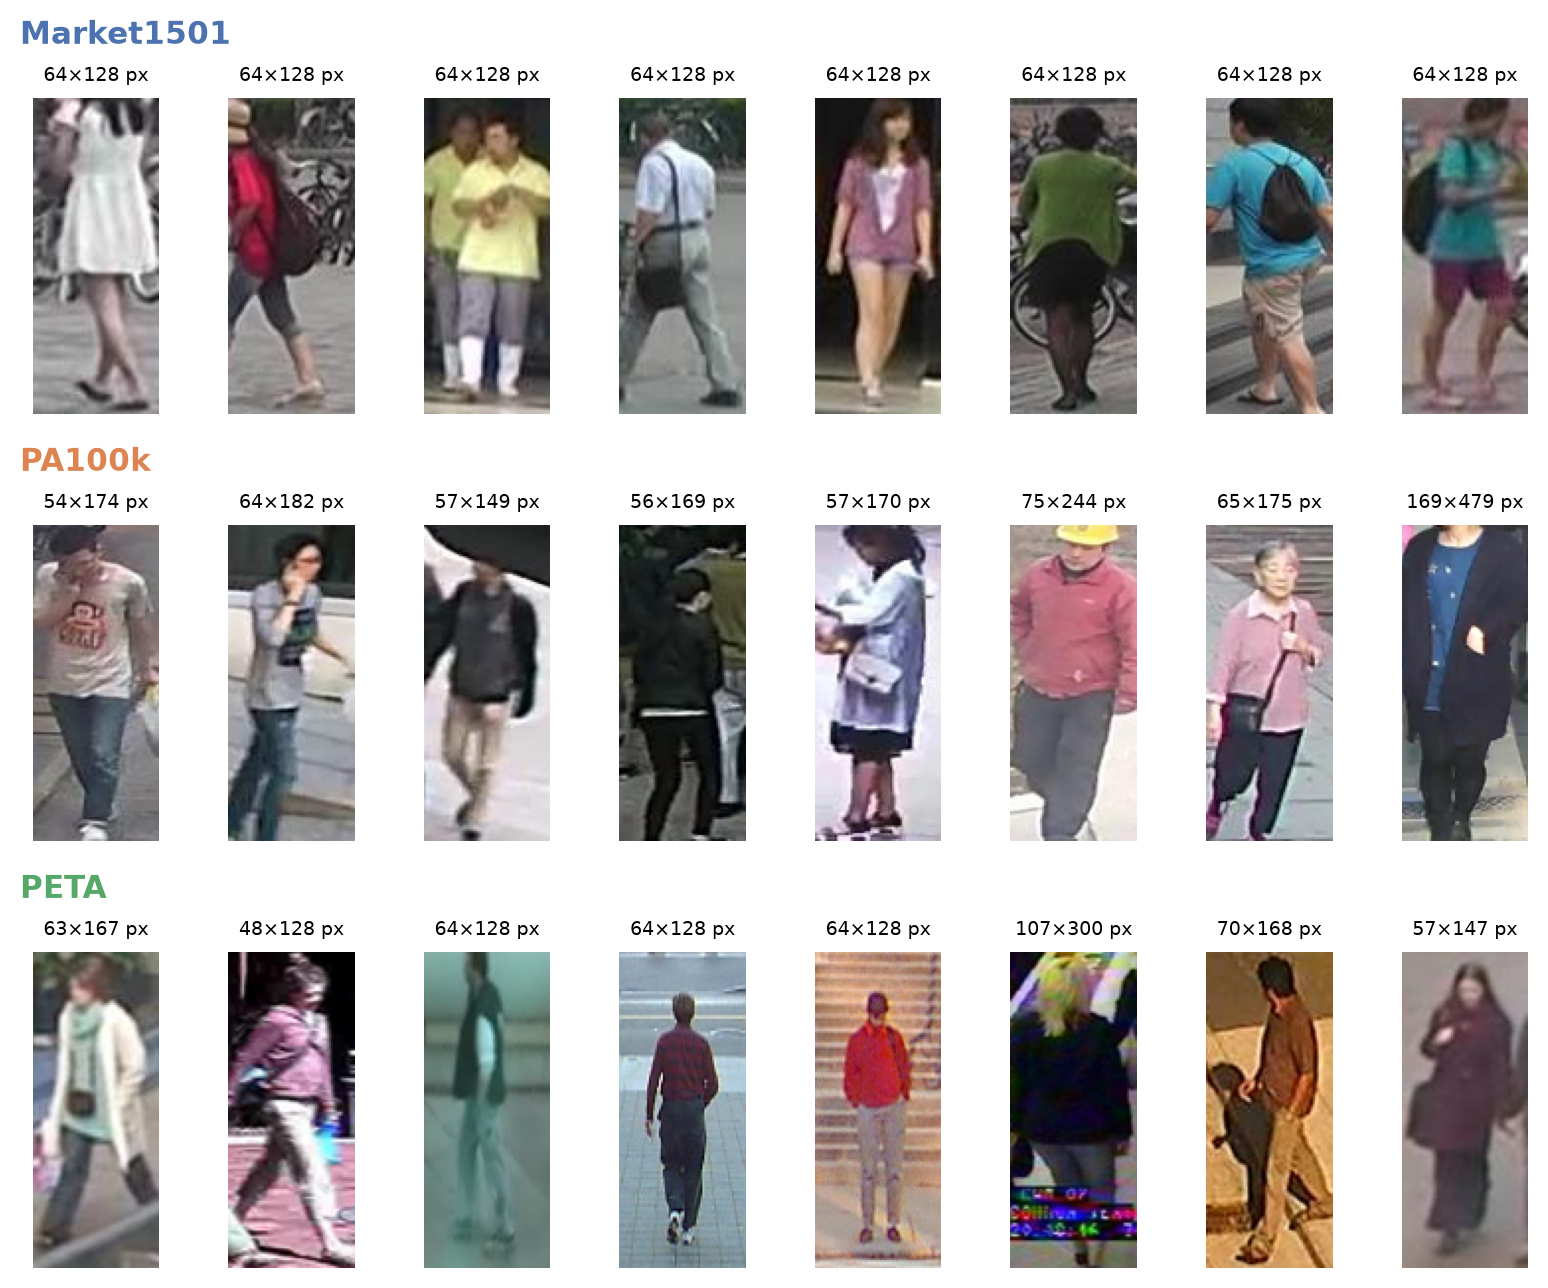
\includegraphics[width=\linewidth]{samples.png}
\caption{Ảnh mẫu ngẫu nhiên từ tập train, hiển thị cùng kích thước, kích thước gốc ghi phía trên. Market1501 có kích thước cố định và bối cảnh đồng nhất trước một siêu thị. PA100k đa dạng về độ phân giải. PETA có chất lượng không đồng đều, nhiều ảnh ám màu hoặc chứa chữ đè từ camera.}
\label{fig:samples}
\end{figure}

\begin{figure}[!htb]
\centering
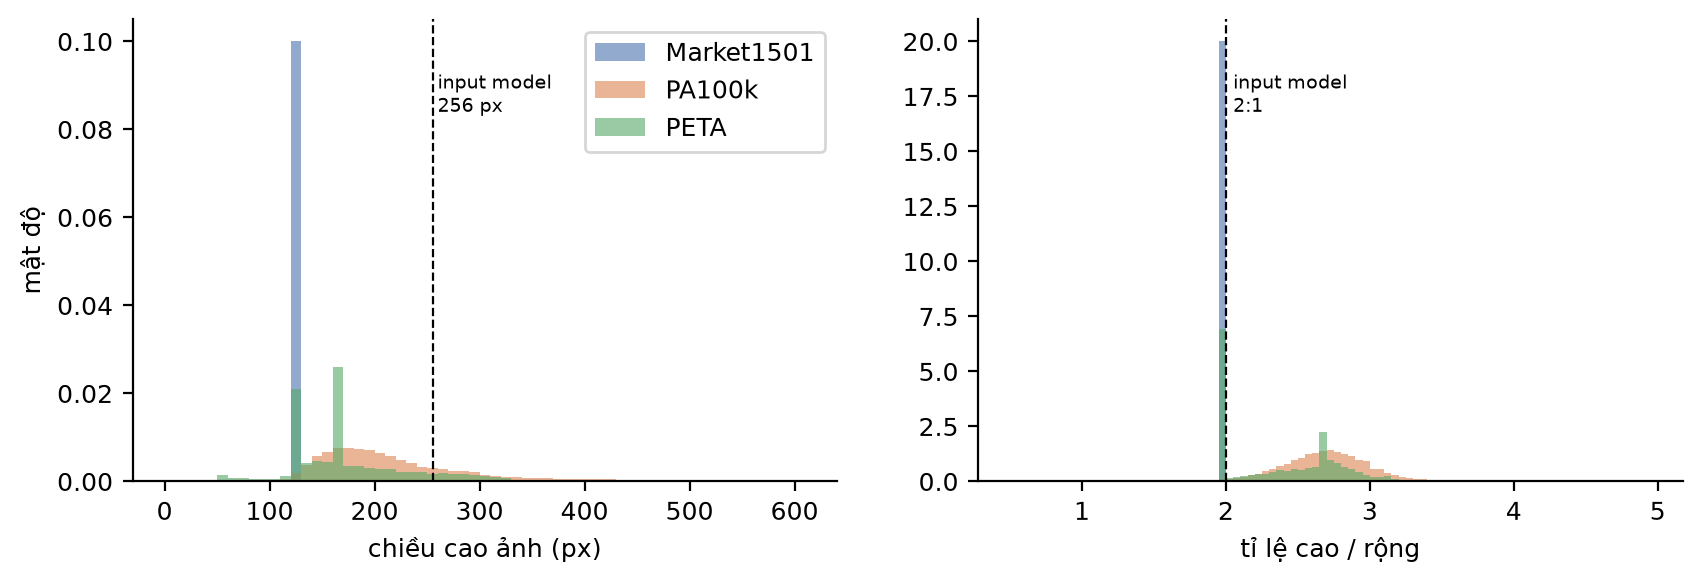
\includegraphics[width=\linewidth]{sizes.png}
\caption{Phân bố chiều cao và tỉ lệ cao/rộng của ảnh. Market1501 là một vạch duy nhất tại 128 pixel và tỉ lệ 2.0. PA100k có tỉ lệ quanh 2.7. Mô hình hiện tại resize mọi ảnh về 256×128, nên ảnh PA100k bị ép ngang và ảnh nhỏ bị phóng to nhiều lần.}
\label{fig:sizes}
\end{figure}

Ảnh test không được công bố. Dựa trên dung lượng file do Codabench báo (379 MB ảnh và 105 KB đáp án đã nén), ước lượng test có khoảng 11 đến 12 nghìn ảnh, trung bình khoảng 33 KB mỗi ảnh. Con số này lớn gấp khoảng 6 lần ảnh val (khoảng 5 KB mỗi ảnh), nên ảnh test có thể có độ phân giải cao hơn dữ liệu train. Đây là ước lượng gián tiếp và chưa được xác nhận.

\subsection{Phân bố nhãn khác nhau giữa các domain}

Hình~\ref{fig:shift} so sánh tỉ lệ ảnh có từng thuộc tính trong ba dataset. Cùng một thuộc tính có thể phổ biến ở domain này và hiếm ở domain khác. UpperBody-Length-Short xuất hiện ở 95\% ảnh Market1501 nhưng chỉ 17\% ảnh PETA, có thể do khác biệt về mùa và khí hậu tại nơi quay. LowerBody-Length-Short chênh lệch từ 62\% xuống 4\%. Một số thuộc tính không có mẫu dương nào trong một dataset, ví dụ Market1501 không có áo nâu, cam, hồng và PETA không có màu Other. Các ô này được coi là chưa gán nhãn và bị bỏ khỏi loss khi huấn luyện.

\begin{figure}[!htb]
\centering
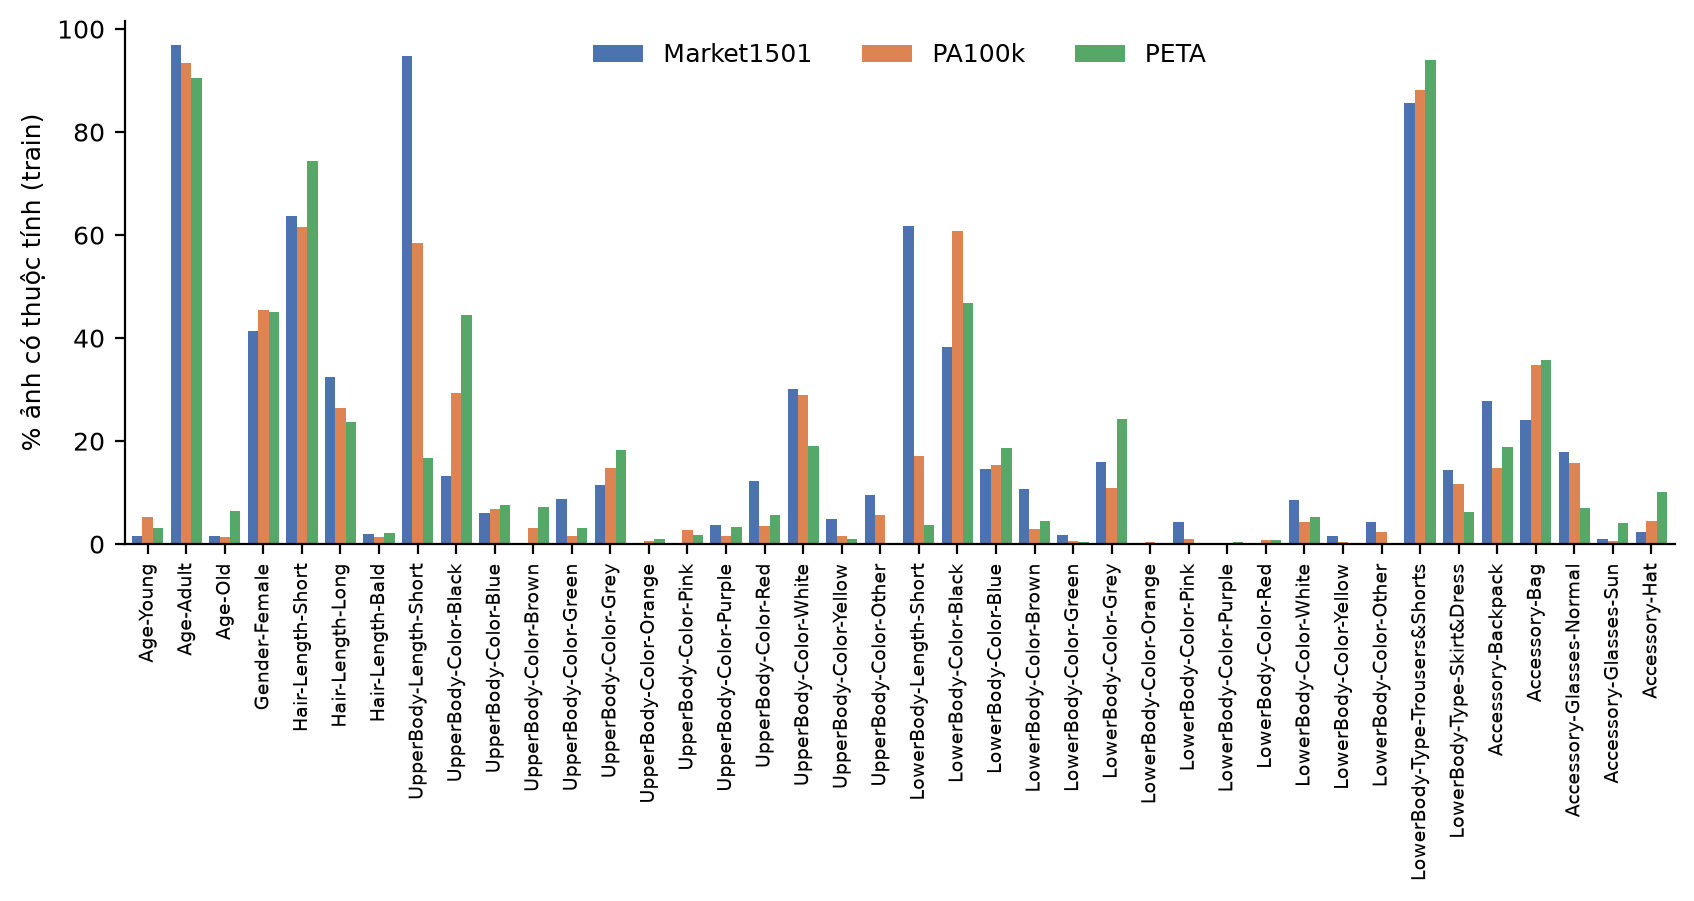
\includegraphics[width=\linewidth]{label_shift.png}
\caption{Tỉ lệ phần trăm ảnh train có từng thuộc tính, tách theo dataset. Chênh lệch lớn giữa các cột cùng thuộc tính cho thấy phân phối nhãn phụ thuộc mạnh vào domain, nên test domain mới gần như chắc chắn có phân phối nhãn khác cả ba.}
\label{fig:shift}
\end{figure}

\subsection{Tương quan giữa các thuộc tính}

Các thuộc tính không độc lập. Trousers\&Shorts và Skirt\&Dress gần như loại trừ nhau. Gender-Female đi kèm Hair-Length-Long, Skirt\&Dress và Accessory-Bag. Mô hình có thể học những tương quan này như một lối tắt. Khi domain mới có tương quan khác, chẳng hạn nhiều phụ nữ tóc ngắn mặc quần dài, lối tắt đó gây lỗi. Báo cáo kỳ 2024 của ban tổ chức nêu hiện tượng này như một nguyên nhân làm mô hình tổng quát kém.

\begin{figure}[!htb]
\centering
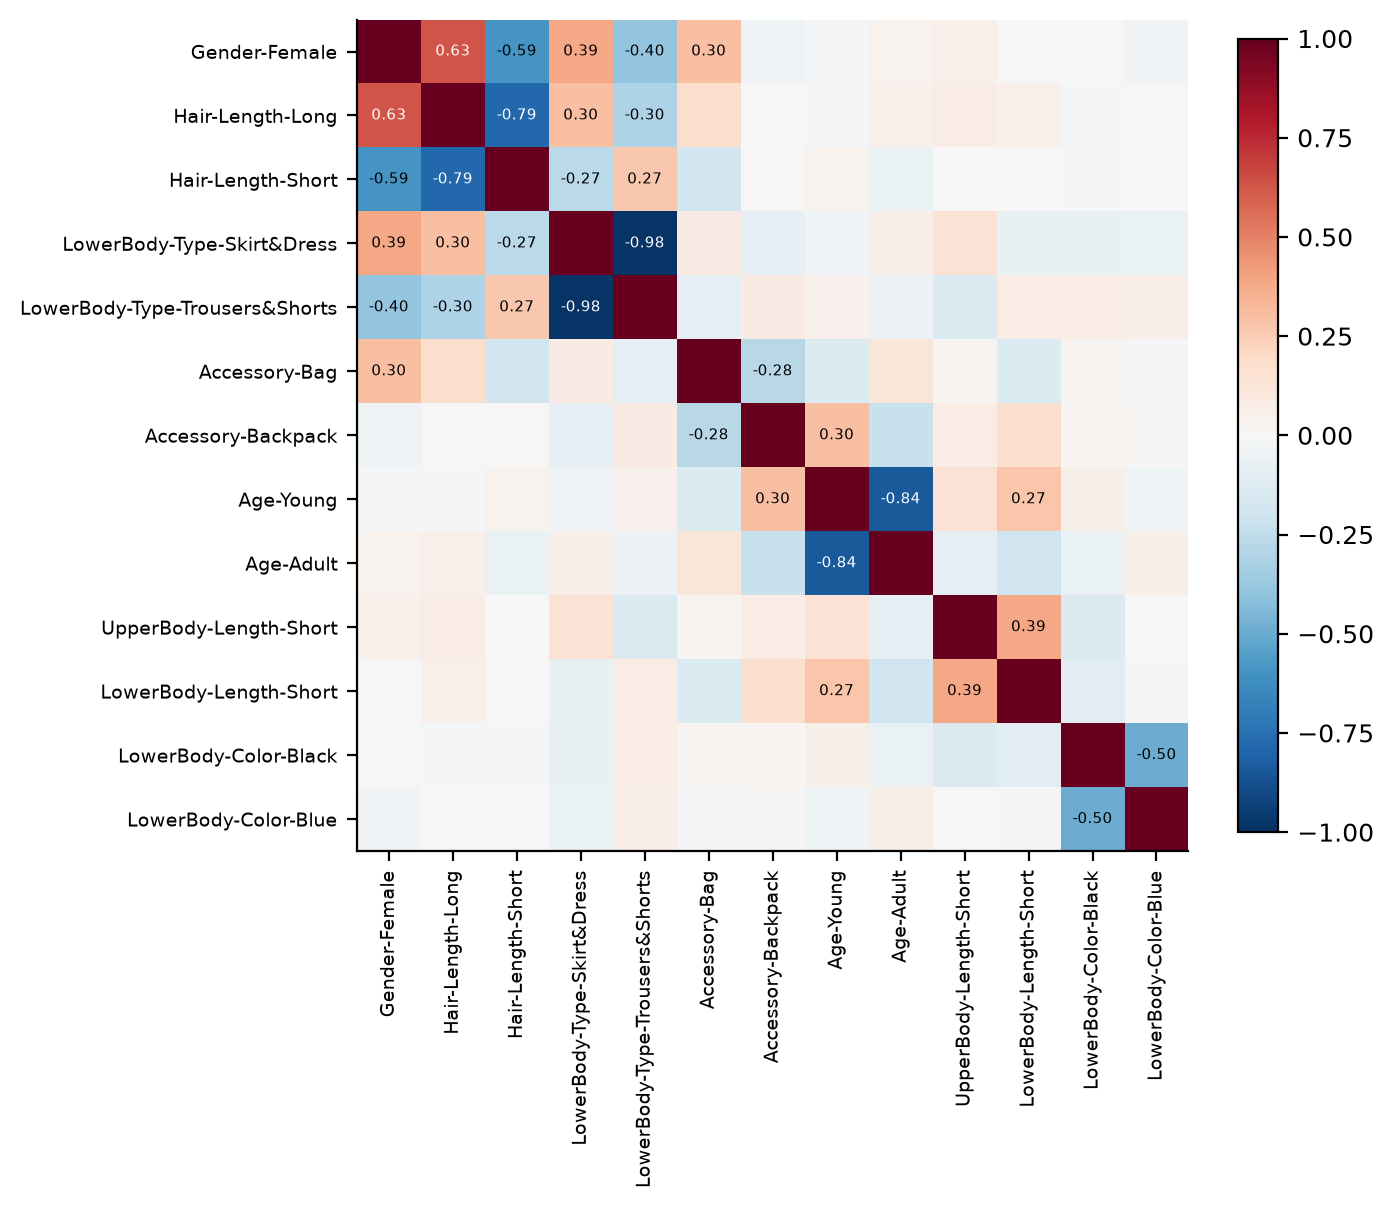
\includegraphics[width=0.52\linewidth]{corr.png}
\caption{Hệ số tương quan giữa một số thuộc tính trên tập train. Các ô có trị tuyệt đối lớn hơn 0.25 được ghi số. Nhóm giới tính, tóc, kiểu quần và túi có tương quan mạnh với nhau.}
\label{fig:corr}
\end{figure}

\subsection{Các trường hợp khó}

Hình~\ref{fig:hard} gom ba loại ảnh khó. Hàng đầu là ảnh nhỏ nhất trong val, cao khoảng 47 đến 52 pixel, ở độ phân giải này kính và màu quần gần như không nhận ra được. Hàng giữa là ảnh PETA bị ám màu, ánh sáng lệch hoặc có khung cắt nằm ngang bất thường. Hàng cuối là những ảnh mô hình dự đoán với độ tin cậy trên 0.99 nhưng trái nhãn. Trong ít nhất ba trên năm ảnh, thuộc tính nhìn thấy trong ảnh khớp với dự đoán của mô hình hơn là với nhãn. Balo, áo đỏ và váy thấy rõ nhưng nhãn bằng 0. Ảnh gán nhãn kính lại chụp từ phía sau nên không thể thấy kính. Nhãn của dữ liệu có nhiễu đáng kể.

\begin{figure}[!htb]
\centering
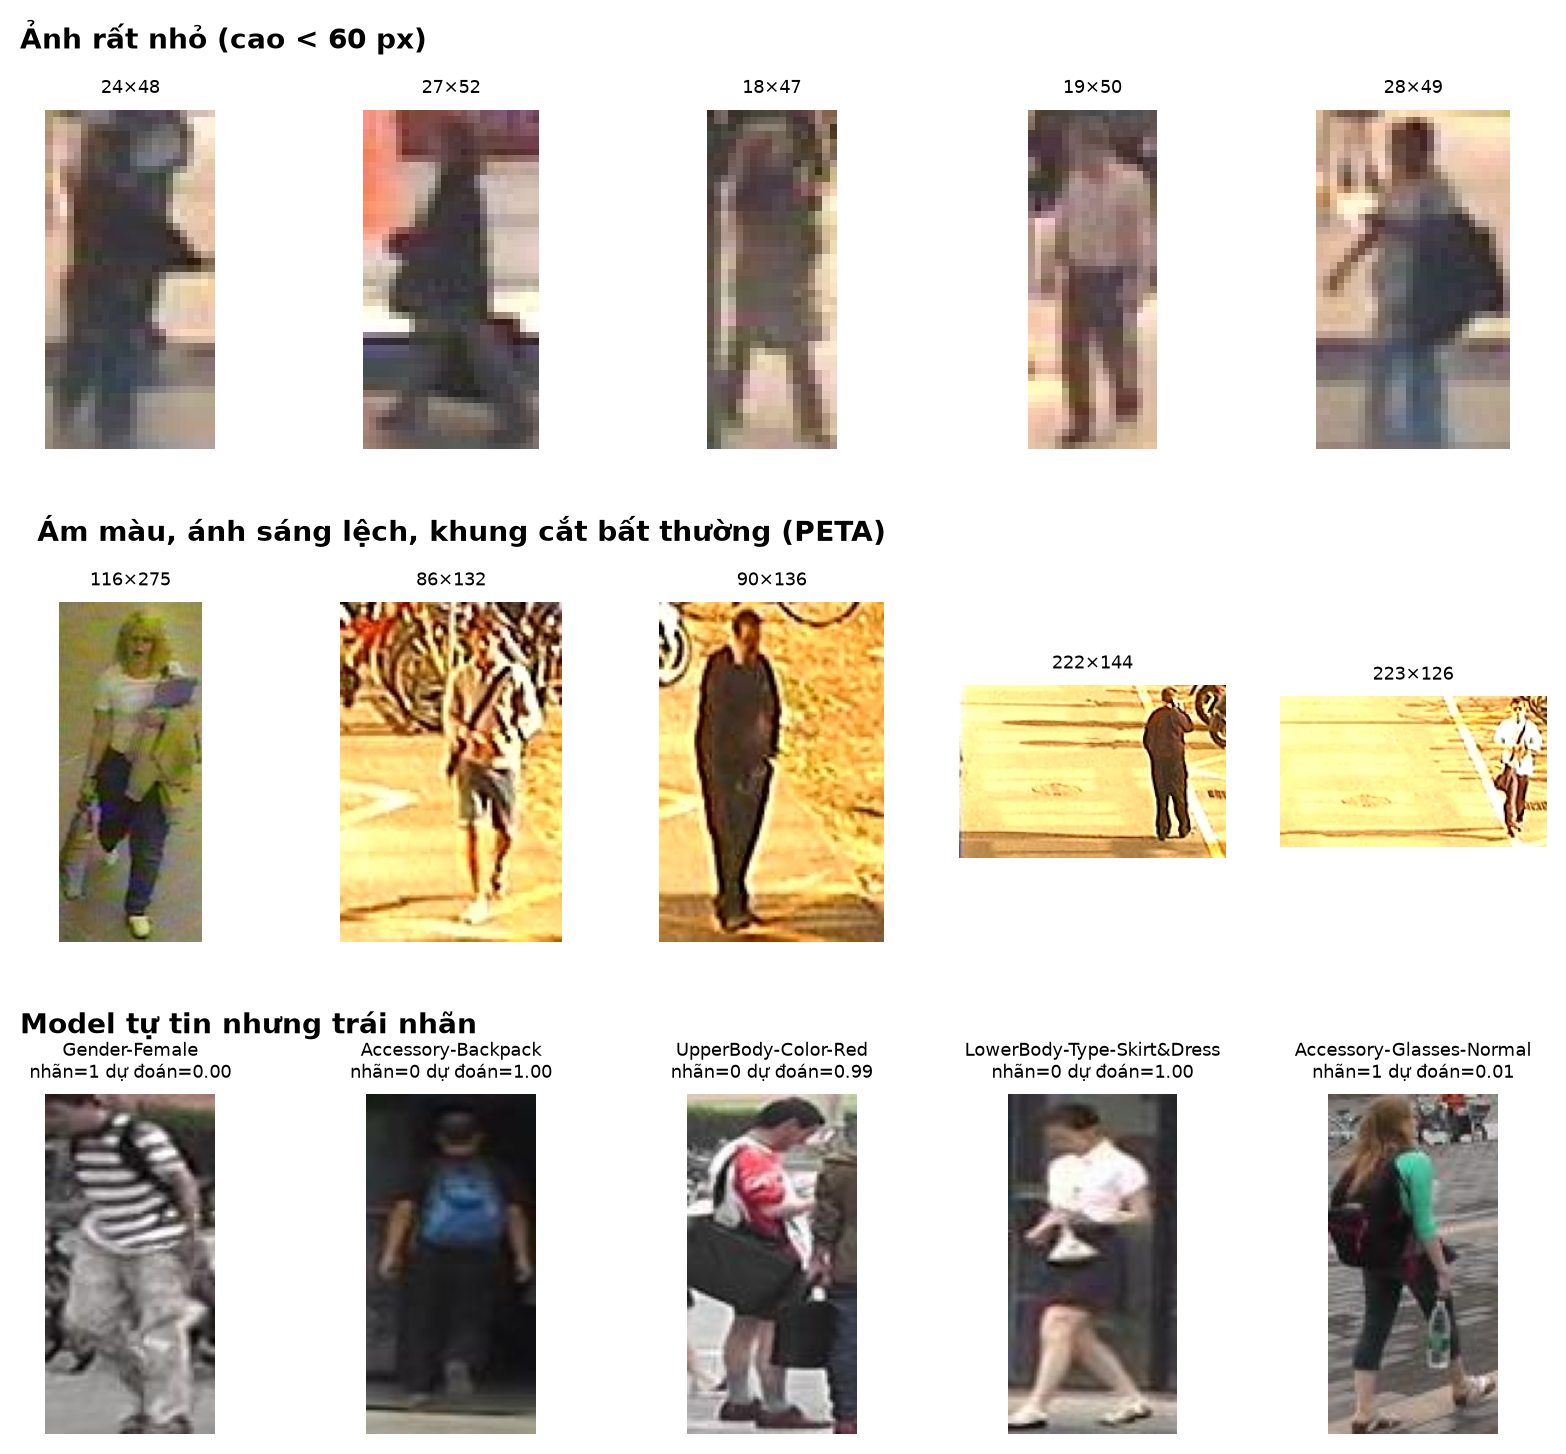
\includegraphics[width=\linewidth]{hard_cases.png}
\caption{Ba nhóm ảnh khó trong tập val. Hàng cuối cho thấy một phần lỗi của mô hình thực ra là lỗi nhãn, nên điểm tối đa đạt được trên dữ liệu này thấp hơn 1.}
\label{fig:hard}
\end{figure}

\section{Vấn đề cần giải quyết}

\subsection{Domain shift giữa dữ liệu train và test}

Đây là vấn đề trung tâm của Track 1. Mô hình hiện tại đạt Challenge\_Avg 0.885 trên val nhưng chỉ 0.777 trên test (Hình~\ref{fig:results}). Val đến từ đúng ba domain đã dùng để huấn luyện nên không phản ánh được năng lực trên domain mới. Khoảng chênh đến từ ba nguồn đã quan sát trong dữ liệu. Nguồn thứ nhất là khác biệt về camera, gồm độ phân giải, màu sắc, góc nhìn. Nguồn thứ hai là khác biệt về phân phối nhãn như mục 4.3. Nguồn thứ ba là khác biệt về tương quan giữa các thuộc tính như mục 4.4.

Hệ quả thực tế là chọn mô hình hay siêu tham số dựa trên val có thể dẫn tới lựa chọn sai. Cần một phép đánh giá mô phỏng domain lạ, ví dụ huấn luyện trên PA100k và Market1501 rồi đánh giá trên PETA.

\subsection{Mất cân bằng nhãn và thuộc tính khó}

Hình~\ref{fig:perattr} xếp 40 thuộc tính theo balanced accuracy trên val. Bốn thuộc tính dưới 80\% gồm Accessory-Glasses-Sun (65\%), UpperBody-Color-Other (70\%), LowerBody-Color-Purple (73\%) và Accessory-Glasses-Normal (77\%). Đây đều là thuộc tính hiếm, hoặc chi tiết nhỏ khó thấy ở độ phân giải thấp, hoặc có định nghĩa mơ hồ như màu Other. Vì mA cho mọi thuộc tính trọng số như nhau, bốn thuộc tính này kéo mA xuống nhiều hơn so với tỉ lệ ảnh của chúng.

\begin{figure}[!htb]
\centering
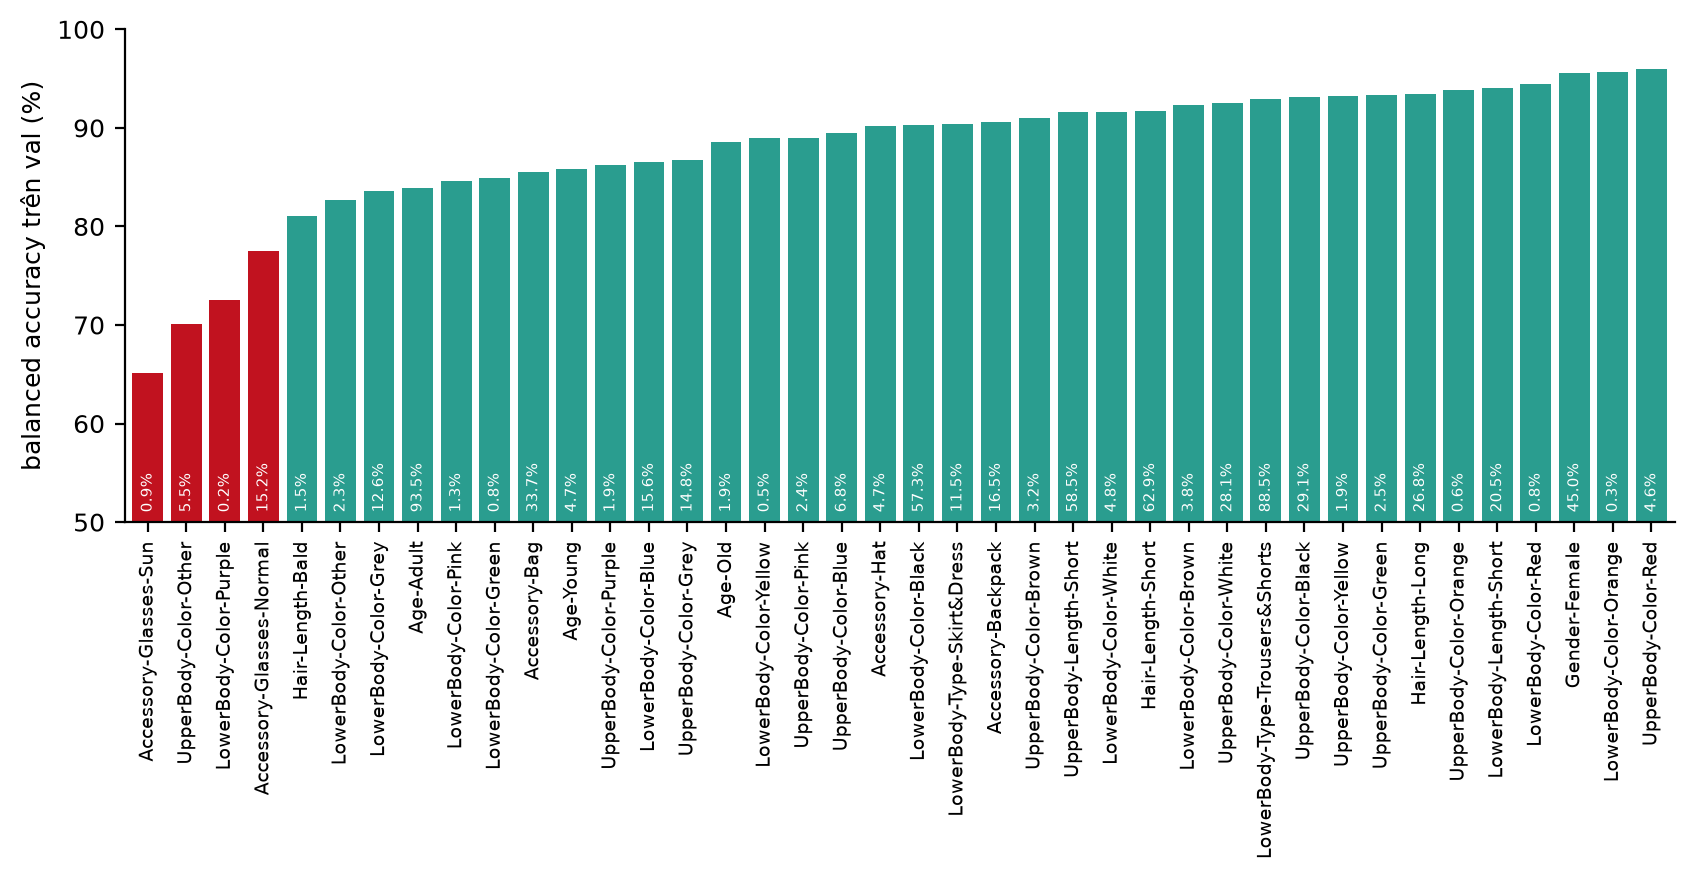
\includegraphics[width=\linewidth]{per_attr.png}
\caption{Balanced accuracy trên val của từng thuộc tính với mô hình hiện tại, trung bình theo dataset. Số trắng trong cột là tỉ lệ ảnh train có thuộc tính đó. Cột đỏ là các thuộc tính dưới 80\%.}
\label{fig:perattr}
\end{figure}

\subsection{Nhiễu nhãn và giới hạn độ phân giải}

Như Hình~\ref{fig:hard}, một phần nhãn trong train và val sai so với nội dung ảnh, và một phần ảnh nhỏ tới mức thuộc tính không còn quan sát được. Mô hình không nên được ép khớp tuyệt đối với các nhãn này. Label smoothing và loss chịu nhiễu là các biện pháp hợp lý.

\subsection{Ràng buộc môi trường chạy}

Bài nộp phải chạy trọn trong 3600 giây trên phần cứng không được công bố và không có log trả về. Lần nộp đầu tiên thất bại mà không rõ nguyên nhân. Phiên bản hiện tại xử lý vấn đề này bằng các cơ chế an toàn gồm tự chuyển sang CPU khi GPU lỗi, dùng số luồng theo giới hạn CPU của container, ngân sách thời gian 45 phút và thay ảnh hỏng bằng ảnh xám. Trên máy thử nghiệm, tốc độ là 4.7 ms mỗi ảnh với GPU và 70 đến 145 ms mỗi ảnh với 2 đến 16 luồng CPU. Ràng buộc này giới hạn kích thước mô hình và số mô hình có thể ensemble.

\section{Tình hình hiện tại}

\subsection{Phương pháp đang dùng}

\begin{table}[H]
\centering\small
\begin{tabularx}{\linewidth}{@{}lX@{}}
\toprule
Thành phần & Cấu hình \\
\midrule
Backbone & DINOv3 ViT-B/16 (86 triệu tham số, pretrain LVD-1689M), input 256×128 \\
Head & Ghép CLS token với trung bình patch token, qua LayerNorm, Dropout và Linear ra 40 logit \\
Loss & Binary cross-entropy có trọng số theo tần suất nhãn, label smoothing 0.05, bỏ qua ô nhãn chưa gán \\
Huấn luyện & AdamW, lr giảm theo độ sâu lớp (hệ số 0.75), cosine 10 epoch, EMA 0.9995, bf16, lấy mẫu cân bằng theo dataset tỉ lệ $\sqrt{N}$ \\
Augmentation & Giả lập độ phân giải thấp, lật ngang, cắt dịch, chỉnh sáng và tương phản không đổi hue, làm mờ, random erasing \\
Hậu xử lý & Offset logit riêng cho từng thuộc tính, fit trên val rồi nhân hệ số 0.6 để giảm rủi ro trên domain lạ \\
Suy luận & TTA lật ngang khi có GPU. Chỉ dùng ảnh gốc khi chạy CPU \\
\bottomrule
\end{tabularx}
\caption{Cấu hình của bài nộp đã được chấm. Dữ liệu huấn luyện chỉ gồm tập train, chưa dùng tập val.}
\end{table}

\subsection{Kết quả}

\begin{table}[H]
\centering\small
\begin{tabular}{@{}lccccc@{}}
\toprule
Tập đánh giá & Challenge\_Avg & mA & Instance-F1 & Inst\_Prec & Inst\_Rec \\
\midrule
Val, Market1501 & 0.886 & 0.877 & 0.895 & 0.884 & 0.912 \\
Val, PA100k & 0.874 & 0.871 & 0.878 & 0.857 & 0.908 \\
Val, PETA & 0.895 & 0.890 & 0.901 & 0.886 & 0.923 \\
Val, trung bình & 0.885 & 0.879 & 0.891 & 0.876 & 0.914 \\
\midrule
Test (leaderboard) & 0.777 & 0.779 & 0.776 & 0.753 & 0.815 \\
\bottomrule
\end{tabular}
\caption{Kết quả của mô hình hiện tại trên val cùng domain và trên test. Mức giảm từ val sang test đồng đều ở cả mA và Instance-F1, khoảng 0.10 đến 0.12 điểm.}
\end{table}

\begin{figure}[!htb]
\centering
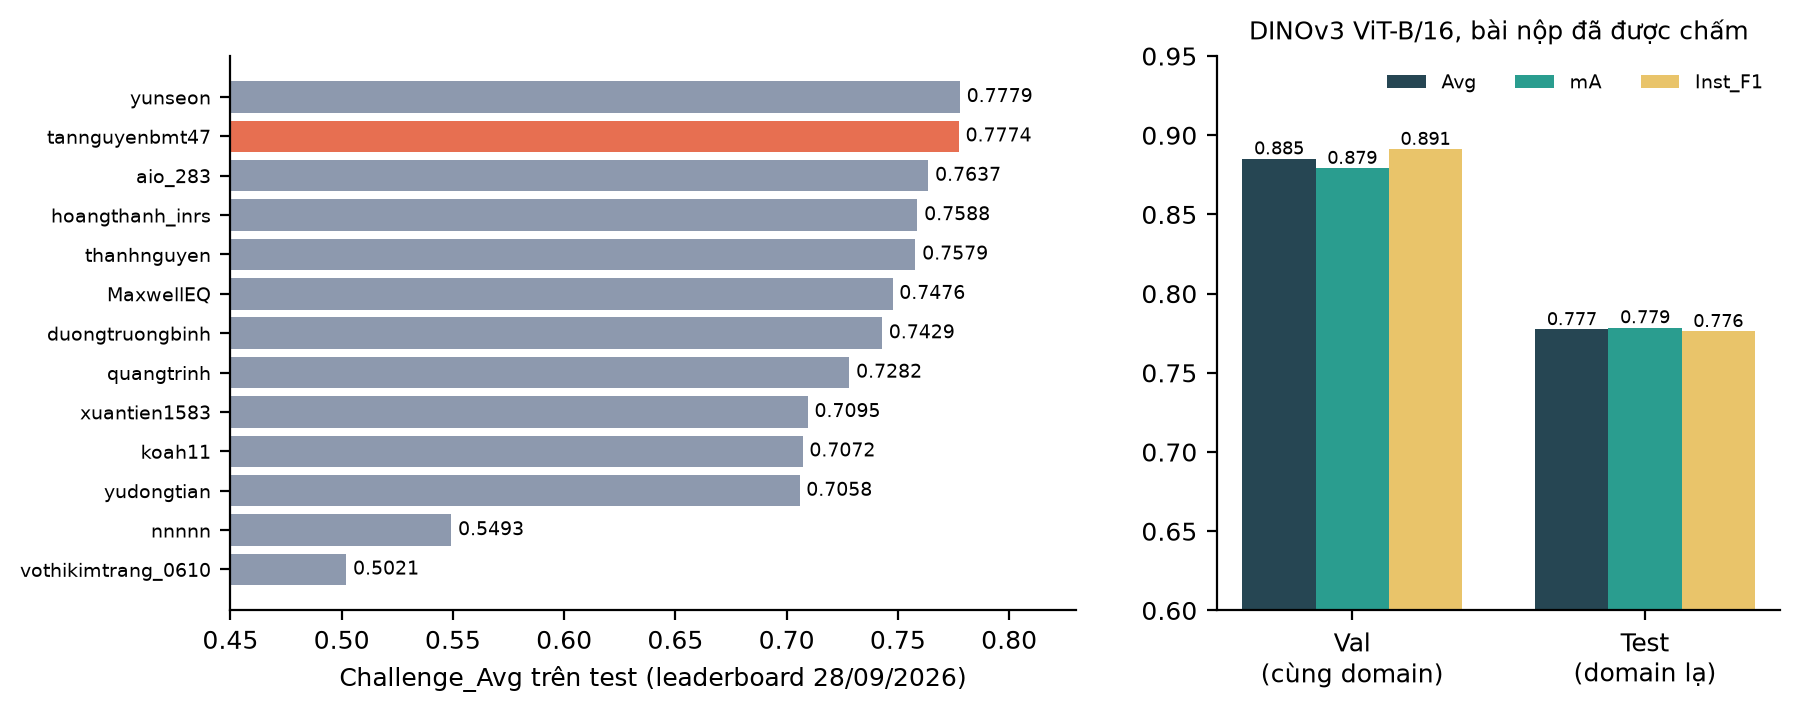
\includegraphics[width=\linewidth]{results.png}
\caption{Bên trái là leaderboard Track 1 ngày 28/09/2026, bỏ các bài có điểm dưới 0.3. Bên phải là cùng một mô hình trên val và test. Ba đội đầu cách nhau chưa tới 0.015 điểm.}
\label{fig:results}
\end{figure}

So với đội dẫn đầu, bài nộp hiện tại có mA gần bằng (0.7786 so với 0.7799) và Instance-F1 gần bằng (0.7762 so với 0.7759). Trên test, precision của bài nộp (0.753) thấp hơn recall (0.815) đáng kể. Điều này gợi ý offset hiện tại vẫn đẩy nhiều thuộc tính lên quá mức trên domain test, và giảm hệ số offset có thể cân lại hai chỉ số.

\section{Hướng tiếp theo}

\begin{enumerate}
\item Dựng phép đánh giá mô phỏng domain lạ bằng cách giữ lại một dataset, dùng nó để chọn mọi siêu tham số thay cho val cùng domain.
\item Fit offset ngưỡng theo cách giữ lại một dataset và thử hệ số offset nhỏ hơn 0.6.
\item Tăng augmentation cho các yếu tố đã quan sát ở mục 4, gồm độ phân giải thấp, nén JPEG, tỉ lệ khung hình, che khuất và ám màu nhẹ.
\item Giữ lại năng lực tổng quát của model pretrain bằng LP-FT, nội suy trọng số kiểu WiSE-FT và SWA.
\item Huấn luyện bản cuối trên cả train và val, thử backbone lớn hơn (ViT-L) và ensemble với một backbone khác loại như CLIP hoặc SigLIP, trong giới hạn thời gian chạy.
\end{enumerate}

\begin{ghichu}
Điểm val không dự đoán được thứ hạng trên test. Mọi cải tiến cần được kiểm chứng trên một domain không có trong dữ liệu huấn luyện trước khi dùng lượt nộp. Leaderboard chỉ giữ bài nộp mới nhất, nên một bài thử nghiệm kém sẽ kéo thứ hạng xuống cho tới lần nộp sau.
\end{ghichu}

\vspace{4pt}
{\small\textbf{Nguồn.} Trang Codabench của cuộc thi (\url{https://www.codabench.org/competitions/18180/}). Starter kit (\url{https://github.com/speckean/UPAR-Challenge-2027}). Specker và cộng sự, UPAR, WACV 2023. Cormier và cộng sự, UPAR Challenge 2023 và 2024, WACV Workshops. Số liệu dữ liệu và kết quả mô hình được tính trực tiếp từ dữ liệu train và val của ban tổ chức.}

\end{document}
